\documentclass[10pt]{beamer}

%% Language and font encodings
\usepackage[english]{babel}
\usepackage[utf8x]{inputenc}
\usepackage[T1]{fontenc}
\usepackage{tikz}
\usetikzlibrary{shapes, snakes}
\usepackage{amsmath}
\usepackage{amssymb}
\usepackage{graphicx}
\usepackage[colorinlistoftodos]{todonotes}
\usepackage[colorlinks=true, allcolors=blue]{hyperref}

%% Sets page size and margins
\usepackage[a4paper,top=2cm,bottom=2cm,left=2cm,right=2cm,marginparwidth=1.00cm]{geometry}
\usetheme{AnnArbor}
\usecolortheme{beaver}

\title{Gravitation: Revision lecture}
\subtitle{Exercise solutions}
\author{Mr. Kwek}
\institute
{ Physics Dept.,\\VJC}
\date{11 Sep 2018}

\begin{document}
%\maketitle
\frame{\titlepage}


\begin{frame}
1(a) The gravitational force acts towards the centre of the Earth.\\
\vspace{10pt}
(b) The Moon moves in the direction perpendicular to the radius with a speed that allows the centripetal acceleration provided by the Earth's gravitational force to keep it along a circular trajectory.  
\end{frame}

\begin{frame}
1(c)\\ \[F=\frac{GMm}{r^2}\]\\
\[F=\frac{6.67\times 10^{-11}\times 6.0 \times 10^{24} \times 7.34 \times 10^{22}}{(3.84 \times 10^8)^2}\]\\
\vspace{10pt}
$F$ = \underline{1.99 $ \times 10^{22}$ N}\\
\end{frame}

\begin{frame}
1(d)The centripetal force required for the circular motion is provided by the force of gravity:\\
Centripetal force = Gravitational force\\
\begin{columns}
\column{0.5\textwidth}
\[mr\omega^2= \frac{GMm}{r^2} \]\\ 
\[\omega= \sqrt{ \frac{GM}{r^3}} \]\\ 
\[ \frac{2\pi}{T}= \sqrt{ \frac{GM}{r^3}} \]\\ 
\column{0.5\textwidth}
\[ \frac{2\pi}{T}= \sqrt{ \frac{6.67\times 10^{-11}\times 6.0 \times 10^{24}}{(3.84 \times 10^8)^3}} \]\\ 
$T = 2.36 \times 10^6 $ s\\ 
\[ T = \frac{2.36 \times 10^6}{3600 \times 24} \]  \\
\vspace{10pt}
$T$ = \underline{27.4 days}\\
\end{columns}
\end{frame}

\begin{frame}
\item 1(e)

\begin{figure}[h]
\centering
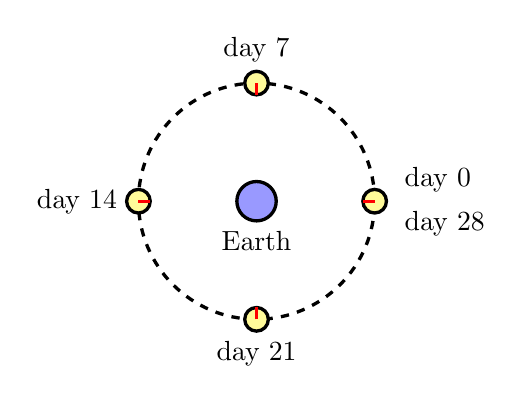
\begin{tikzpicture}[scale=0.5]
%\draw[help lines, color=gray!30, thick] (-4.9,-4.9) grid (4.9,4.9);
\filldraw [fill=blue!40, very thick] (0,0) circle (0.5cm);
\node (earth) at (0,-1) {Earth};

\draw [very thick, dashed] (0,0) circle (3cm);
\filldraw [fill=yellow!40, very thick] (3,0) circle (0.3cm);
\draw [very thick, red] (3,0) -- (2.7,0);
\node[anchor = south west] (moon1) at (3,0) {\hspace{4pt} day 0};
\node[anchor = north west] (moon5) at (3,0) {\hspace{4pt} day 28};

\filldraw [fill=yellow!40, very thick] (0,3) circle (0.3cm);
\draw [very thick, red] (0,3) -- (0,2.7);
\node[anchor = south] (moon2) at (0,3.3) {day 7};

\filldraw [fill=yellow!40, very thick] (-3,0) circle (0.3cm);
\draw [very thick, red] (-3,0) -- (-2.7,0);
\node[anchor = east] (moon3) at (-3.3,0) {day 14};

\filldraw [fill=yellow!40, very thick] (0,-3) circle (0.3cm);
\draw [very thick, red] (0,-3) -- (0,-2.7);
\node[anchor = north] (moon4) at (0,-3.3) {day 21};

\end{tikzpicture}
\caption{Observer on Earth sees the same face of the Moon at all times}
\label{fig:moon_orbit}
\end{figure}


If a terrestrial observer sees the same face of the Moon all the time, the Moon must be rotating about its own axis at the exact same rate as its orbital motion around the Earth.\\ Hence, rotational period of Moon = \underline{27.4 days}. 
\end{frame}

\begin{frame}
1(f)
\begin{figure}[h]
    \centering
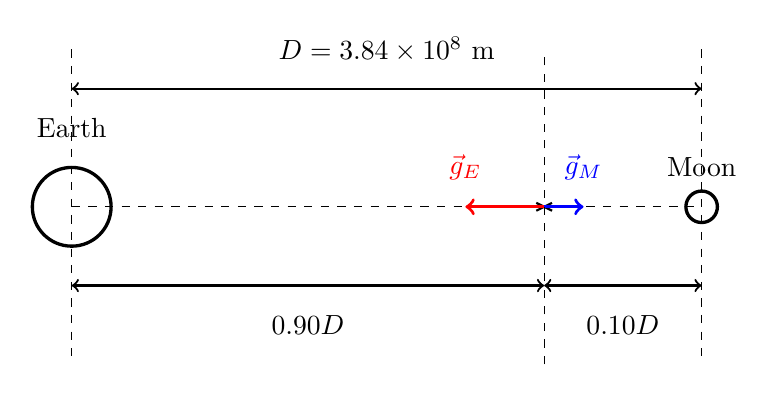
\begin{tikzpicture}
\coordinate (x) at (2,0);
%\draw[help lines, color=gray!30, thick] (-4.9,-4.9) grid (4.9,4.9);
\draw [very thick] (-4,0) circle (0.5cm);
\draw [dashed] (-4,0) -- (4,0);
\draw [thick] (x) -- (2.1,0.05);
\draw [thick] (x) -- (2.1,-0.05);
\draw [thick] (x) -- (1.9,0.05);
\draw [thick] (x) -- (1.9,-0.05);
\draw [->,very thick,blue] (x) -- (2.5,0);
\node [color=blue] (g_moon) at (2.5,0.5) {$\vec{g}_{M}$};
\draw [->,very thick, red] (x) -- (1.0,0);
\node [color=red] (g_earth) at (1,0.5) {$\vec{g}_E$};
\draw [dashed] (-4,2) -- (-4,-2);
\draw [dashed] (2,-2) -- (2,2);
\draw [<->, thick] (-4,1.5) -- (4,1.5);
\node (D) at (0,2) {$D = 3.84 \times 10^8$ m};
\draw [<->, thick] (2,-1) -- (4,-1);
\node (d2) at (3,-1.5) {$0.10 D$};
\draw [<->, thick] (2,-1) -- (-4,-1);
\node (d1) at (-1,-1.5) {$0.90 D$};
\draw [dashed] (4,2) -- (4,-2);

\node (earth) at (-4,1) {Earth};
\draw [very thick] (4,0) circle (0.2cm);
\node (moon) at (4,0.5) {Moon};
\end{tikzpicture}
    \caption{Gravitational field at a point between Earth and Moon}
    \label{fig:halley}
\end{figure}

Resultant grav. field at point = $g = g_M - g_E$ \\
\[ g = \frac{GM_m}{x_m^2} -  \frac{GM_E}{x_E^2}\] \\
, taking the Earth-to-Moon direction as positive.\\
\end{frame}

\begin{frame}
1(f) (continued)
\[ g = \frac{6.67\times 10^{-11}\times  7.34 \times 10^{22}}{(0.1 \times 3.84 \times 10^8)^2} -  \frac{6.67\times 10^{-11}\times 6.0 \times 10^{24}} {(0.9 \times 3.84 \times 10^8)^2}\]
\vspace{10pt}
$g = \underline{-3.1 \times 10^{-5}$ N kg$^{-1}}$\\
\vspace{10pt}
Hence, the resultant gravitational field at the point is \underline{$3.1 \times 10^{-5}$ N kg$^{-1}$ and acts towards the Earth}.
\end{frame}

\begin{frame}
1(g) 
Resultant grav. potential at point = $\phi = \phi_M + \phi_E$ \\
\[ \phi = \left( -\frac{GM_m}{x_m} \right) + \left(-\frac{GM_E}{x_E} \right) \] \\
\[ \phi = \left( -\frac{6.67\times 10^{-11}\times  7.34 \times 10^{22}}{(0.1 \times 3.84 \times 10^8)} \right) + \left(-\frac{6.67\times 10^{-11}\times 6.0 \times 10^{24}} {(0.9 \times 3.84 \times 10^8)} \right) \]
\vspace{10pt}
$\phi = \underline{-1.3 \times 10^{6} $ J kg$^{-1}}$\\
\vspace{10pt}
Hence, the resultant potential at the point is $-1.3 \times 10^6$ J kg$^{-1}$.

\end{frame}


\begin{frame}
2(a) Grav. field at surface, $g$ = 3.71 m s$^{-2}$
\[ g = \frac{GM}{R^2} \] 
\[\therefore 3.71 = \frac{6.67 \times 10^{-11} \times M}{(3390,000)^2} \] \\
Hence, the mass of Mars is:\\
\vspace{10pt}
$M = \underline{6.39 \times 10^{23}}$ kg  \\
\end{frame}

\begin{frame}
2(b) Centripetal force required = Grav. force acting on spacecraft \\
\vspace{10pt}
\begin{columns}
\column{0.5\textwidth}
\[ \frac{mv^2}{r}=\frac{GMm}{r^2}    \]
\[v = \sqrt{\frac{GM}{r}}    \]
\[v = \sqrt{\frac{6.67 \times 10^{-11} \times 6.39 \times 10^{23}}{3390,000+300,000}}    \]
$\therefore v$=\underline{3410 m s$^{-1}$ }\\
\column{0.5\textwidth}
The period $T$ is the time taken for the spacecraft to complete one circular orbit.\\
\[ T =\frac{2\pi r}{v}   \]
\[ T =\frac{2\pi (3390,000+300,000)}{3410}   \]
$\therefore T = \underline{6810}$ s\\
\end{columns}
\end{frame}

\begin{frame}
2(c)
\[g=\frac{GM}{r^2}   \]
\[g=\frac{6.67 \times 10^{-11} \times 6.39 \times 10^{23}}{(3390,000+300,000)^2}   \]
$\therefore g$ = \underline{3.15 N kg$^{-1}$} \\
\vspace{15pt}
2(d) By definition,\\
\[ g = \frac{F}{m}   \]
$\therefore F = m \times g = 0.020 \times 3.15$\\
\vspace{10pt}
$\therefore F = \underline{0.063} $ N\\

\end{frame}

\begin{frame}
2(e) For a synchronous orbit,\\ the orbital period = planet rotational period.\\
$T$ = 1.026 days\\
Centripetal force required = Grav. force acting on spacecraft \\
\[ mr \omega^2 =\frac{GMm}{r^2}    \]
\[r^3 \omega^2 = GM  \]
\[r^3 \left( \frac{2\pi}{T} \right)^2 = GM    \]
\[r^3 \left( \frac{2\pi}{1.026\times 24 \times 3600} \right)^2 = 6.67 \times 10^{-11} \times 6.39 \times 10^{23} \]
$\therefore r = \underline{2.04 \times 10^7}$\underline{ m}\\
\end{frame}

\begin{frame}
2(f) Grav. potential at a point in the initial orbit is:\\
\[\phi_1 = -\frac{GM}{r_1}  \]
\[\phi_1 = -\frac{6.67 \times 10^{-11} \times 6.39 \times 10^{23}}{3390,000+300,000} \]
\vspace{10pt}
$\phi_1 = \underline{-1.16 \times 10^7}$ \underline{J kg$^{-1}$}\\
\end{frame}

\begin{frame}
2(g) Net work done by external force (due to rocket) = Change in total energy\\
But, total energy = KE + GPE\\
\[E=\frac{1}{2} mv^2 + \left( -\frac{GMm}{r} \right)   \]
\[E=\frac{GMm}{2r} + \left( -\frac{GMm}{r} \right)   \]
, via $\frac{mv^2}{r}=\frac{GMm}{r^2} $
\[E=-\frac{GMm}{2r} \] 
$\therefore W = E_2 - E_1$\\
\[W= \left( -\frac{GMm}{2r_2} \right) - \left( -\frac{GMm}{2r_1} \right)   \] 
\end{frame}

\begin{frame}
\[W= \frac{GMm}{2} \left( \frac{1}{r_1} - \frac{1}{r_2} \right) \] 
\[W= \frac{6.67 \times 10^{-11} \times 6.39 \times 10^{23} \times 2180}{2} \left( \frac{1}{3390,000+300,000} - \frac{1}{2.04 \times 10^7} \right) \] 
$W = \underline{1.03 \times 10^{10}}$ J \\
\end{frame}

\begin{frame}
2(h) By the Law of Conservation of Energy,\\
Total energy at initial position = Total energy at final position (surface)\\
$KE_1 + GPE_1 = KE_2 + GPE_2 $\\
\[0 + \left( -\frac{GMm}{r_1} \right) = \frac{1}{2}mv^2 + \left( -\frac{GMm}{R} \right)   \]
\[\frac{1}{2}mv^2 = GMm \left( \frac{1}{R}  -\frac{1}{r_1} \right) \]
\[v = \sqrt{2GM \left( \frac{1}{R}  -\frac{1}{r_1} \right) } \]
\end{frame}

\begin{frame}
\[v = \sqrt{2 \times 6.67 \times 10^{-11} \times 6.39 \times 10^{23} \left( \frac{1}{3390,000}  -\frac{1}{2.04 \times 10^7} \right) } \]
\vspace{10pt}
$v = \underline{4580$ m s$^{-1}}$ \\
\end{frame}

\begin{frame}
2(i) For mass (metal fragment) to reach just infinity,\\
by the Law of Conservation of Energy,\\
initial total energy $\ge$ total energy of stationary mass at infinity.\\
$ KE_1 + GPE_1 \ge KE_{\infty} + GPE_{\infty} $ \\
\[\frac{1}{2}mv^2 +  \left( -\frac{GMm}{r_1} \right) \ge 0 + 0  \]
\[\frac{1}{2}mv^2 \ge  \frac{GMm}{r_1} \]
\[ v \ge \sqrt{\frac{2GM}{r_1}}    \]
\[ v \ge \sqrt{\frac{2 \times 6.67 \times 10^{-11} \times 6.39 \times 10^{23}}{2.04 \times 10^7}}    \]
$v$ = \underline{2040 m s$^{-1}$} \\
\end{frame} 


\begin{frame}
3(a)
\[\phi_1 = -\frac{GM}{r_1}  \]
\[\phi_1 = -\frac{6.67 \times 10^{-11} \times 1.99 \times 10^{30}}{0.586 \times 1.50 \times 10^{11}}  \]
\vspace{10pt}
$ \phi_1 = \underline{-1.51 \times 10^9} $ \underline{J kg $^{-1}$} \\
\vspace{10pt}
3(b)
\[\phi_2 = -\frac{GM}{r_2}  \]
\[\phi_2 = -\frac{6.67 \times 10^{-11} \times 1.99 \times 10^{30}}{35.1 \times 1.50 \times 10^{11}}  \]
\vspace{10pt}
$ \phi_2 = \underline{-2.52 \times 10^7} $ \underline{J kg $^{-1}$ }\\
\end{frame}

\begin{frame}
3(c)
By the Law of Conservation of Energy,\\
total energy at perihelion = total energy at aphelion \\
$KE_1 + GPE_1 = KE_2 + GPE_2 $\\
\[ \frac{1}{2}mv_1^2 + m \phi_1 =  \frac{1}{2}mv_2^2 + m \phi_2   \]
\[ \frac{1}{2}v_1^2 + \phi_1 =  \frac{1}{2}v_2^2 + \phi_2   \]
\[ \frac{1}{2}\times 70560^2 + (-1.51 \times 10^9) =  \frac{1}{2}v_2^2 + (-2.52 \times 10^7)   \]
\vspace{10pt}
$ v_2$ = \underline{44820 m s$^{-1}$} \\

\end{frame}


\end{document}
